\chapter[Analiza zmogljivosti obla"cne storitve DigitalOcean]{Analiza zmogljivosti obla"cne storitve DigitalOcean}

\pagestyle{fancy}
\fancyhf{}
\fancyhead[LE,RO]{\thepage}
\fancyhead[RE,LO]{\leftmark}
\lstset{language=C}

\huge "Ziga Kokelj, Tadej Hiti,\\Miha Bizjak, Matej Kristan
\normalsize
\bigskip

\section{Opis problema} \label{8_opis_problema}
\noindent V zadnjem desetletju se na vseh podro"cjih ra"cunalni"stva vse bolj uveljavljajo obla"cne storitve in koncept odjemalec - stre"znik (angl. \textit{client - server}). Z ve"canjem hitrosti internetnih povezav kon"cne delovne to"cke (predvsem osebni ra"cunalniki) izgubljajo del svojih primarnih funkcij. Hranjenje in obdelavo podatkov vse bolj prepu"s"cajo obla"cnim storitvam. V na"si analizi smo se osredoto"cili na obdelavo podatkov na strani stre"znika. Za breme smo izbrali datoteke razli"cnih velikosti, ki vsebujejo naklju"cna "stevila. Te datoteke odjemalci po"sljejo na stre"znik, ta pa jih uredi v nara"s"cajo"cem vrstnem redu in po"slje nazaj. Na sliki \ref{8_opis_problema} je grafi"cen prikaz opisanega problema. Na"se testiranje bo obsegalo merjenje  "casov "cakanja  odjemalcev na urejeno datoteko ter merjenje obremenjenosti stre"znika.

\begin{figure}
  \centering
    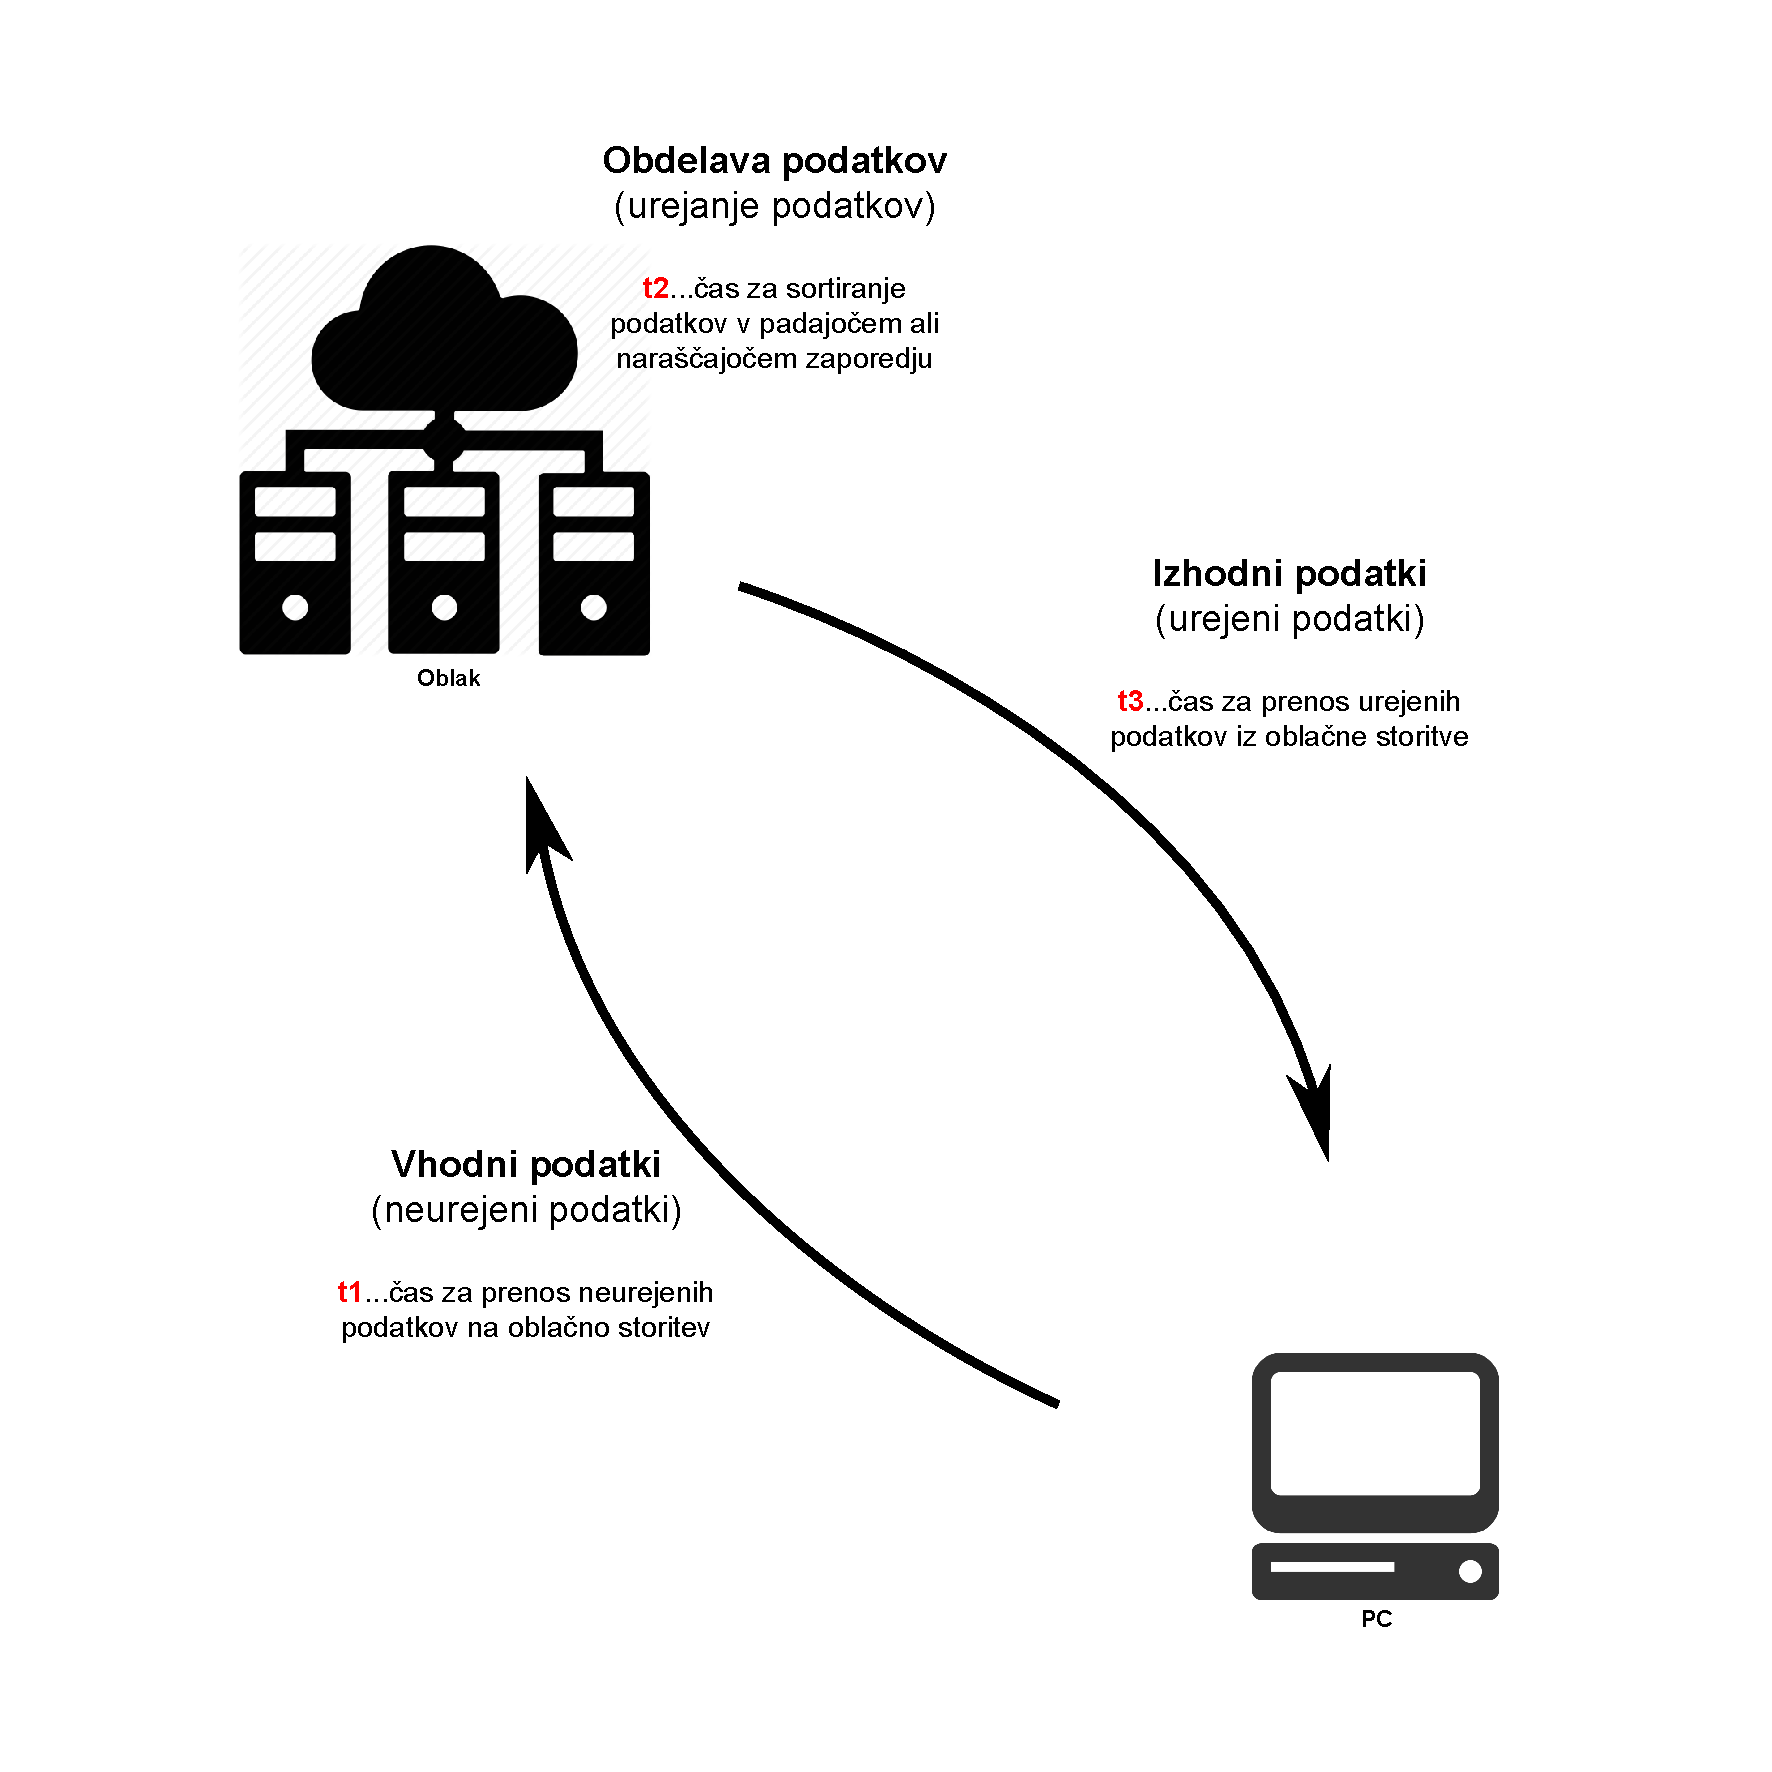
\includegraphics[width=0.74\textwidth]{8_zzrs_opis_problema.pdf}
  \caption{Shema delovanja sistema.}
  \label{8_opis_problema}
\end{figure}


\section{Izbira tehnologij in algoritmov}
V tem razdelku so opisane tehnologije in algoritmi, ki smo jih uporabili za na"so analizo.


\subsection{Tehnologija na strani stre"znika }
Na obla"cni storitvi smo implementirali stre"znik, ki je realiziran v jeziku JavaScript \cite{8_js} z uporabo knji"znice Node.js \cite{8_node}. Stre"znik "caka na HTTP zahteve s strani klienta, kateri po"slje datoteko "stevil za urejanje. Ob sprejemu datoteke s strani stre"znika se za"cne izvajati program, ki "stevila v datoteki uredi v nara"s"cajo"cem vrstnem redu. Ker je za namene testiranja obla"cne infrastrukture bistveno, da se program "cim hitreje izvr"si smo za ta namen uporabili programski jezik C \cite{8_c}, ki spada med najhitrej"se programske jezike, zaradi njegove nizko-nivojske lege na procesorski arhitekturi. Po kon"canem sortiranju stre"znik urejeno datoteko po"slje nazaj odjemalcu.

\subsection{Tehnologija za avtomatizacijo odjemalcev}
Zaradi avtomatskega testiranja smo napisali skripto v programskem jeziku Python \cite{8_py}, ki omogo"ca avtomatsko po"siljanje datotek na stre"znik, ter "caka na odgovor(urejeno datoteko s "stevili). Ob tem zabele"zimo "se "cas pred po"siljanjem zahteve in "cas po prejetju urejene datoteke, da dobimo celotni "cas potreben za po"siljanje in sortiranje na stre"zniku. Ker je odjemalcev lahko ve"cje "stevilo, smo ta problem re"sili z nitmi, kjer vsaka nit predstavlja enega odjemalca in po"silja zahteve na stre"znik preko istega IP naslova.

\subsection{Generiranje vhodnih podatkov}
V programskem jeziku C smo napisali generator datotek, ki ustvari datoteko "zeljene velikosti z naklju"cnimi "stevili. Za teste smo generirali datoteke velikosti 10000, 20000, 30000, 40000 in 50000 "stevil tipa integer.

\begin{figure} [!h]
  \centering
    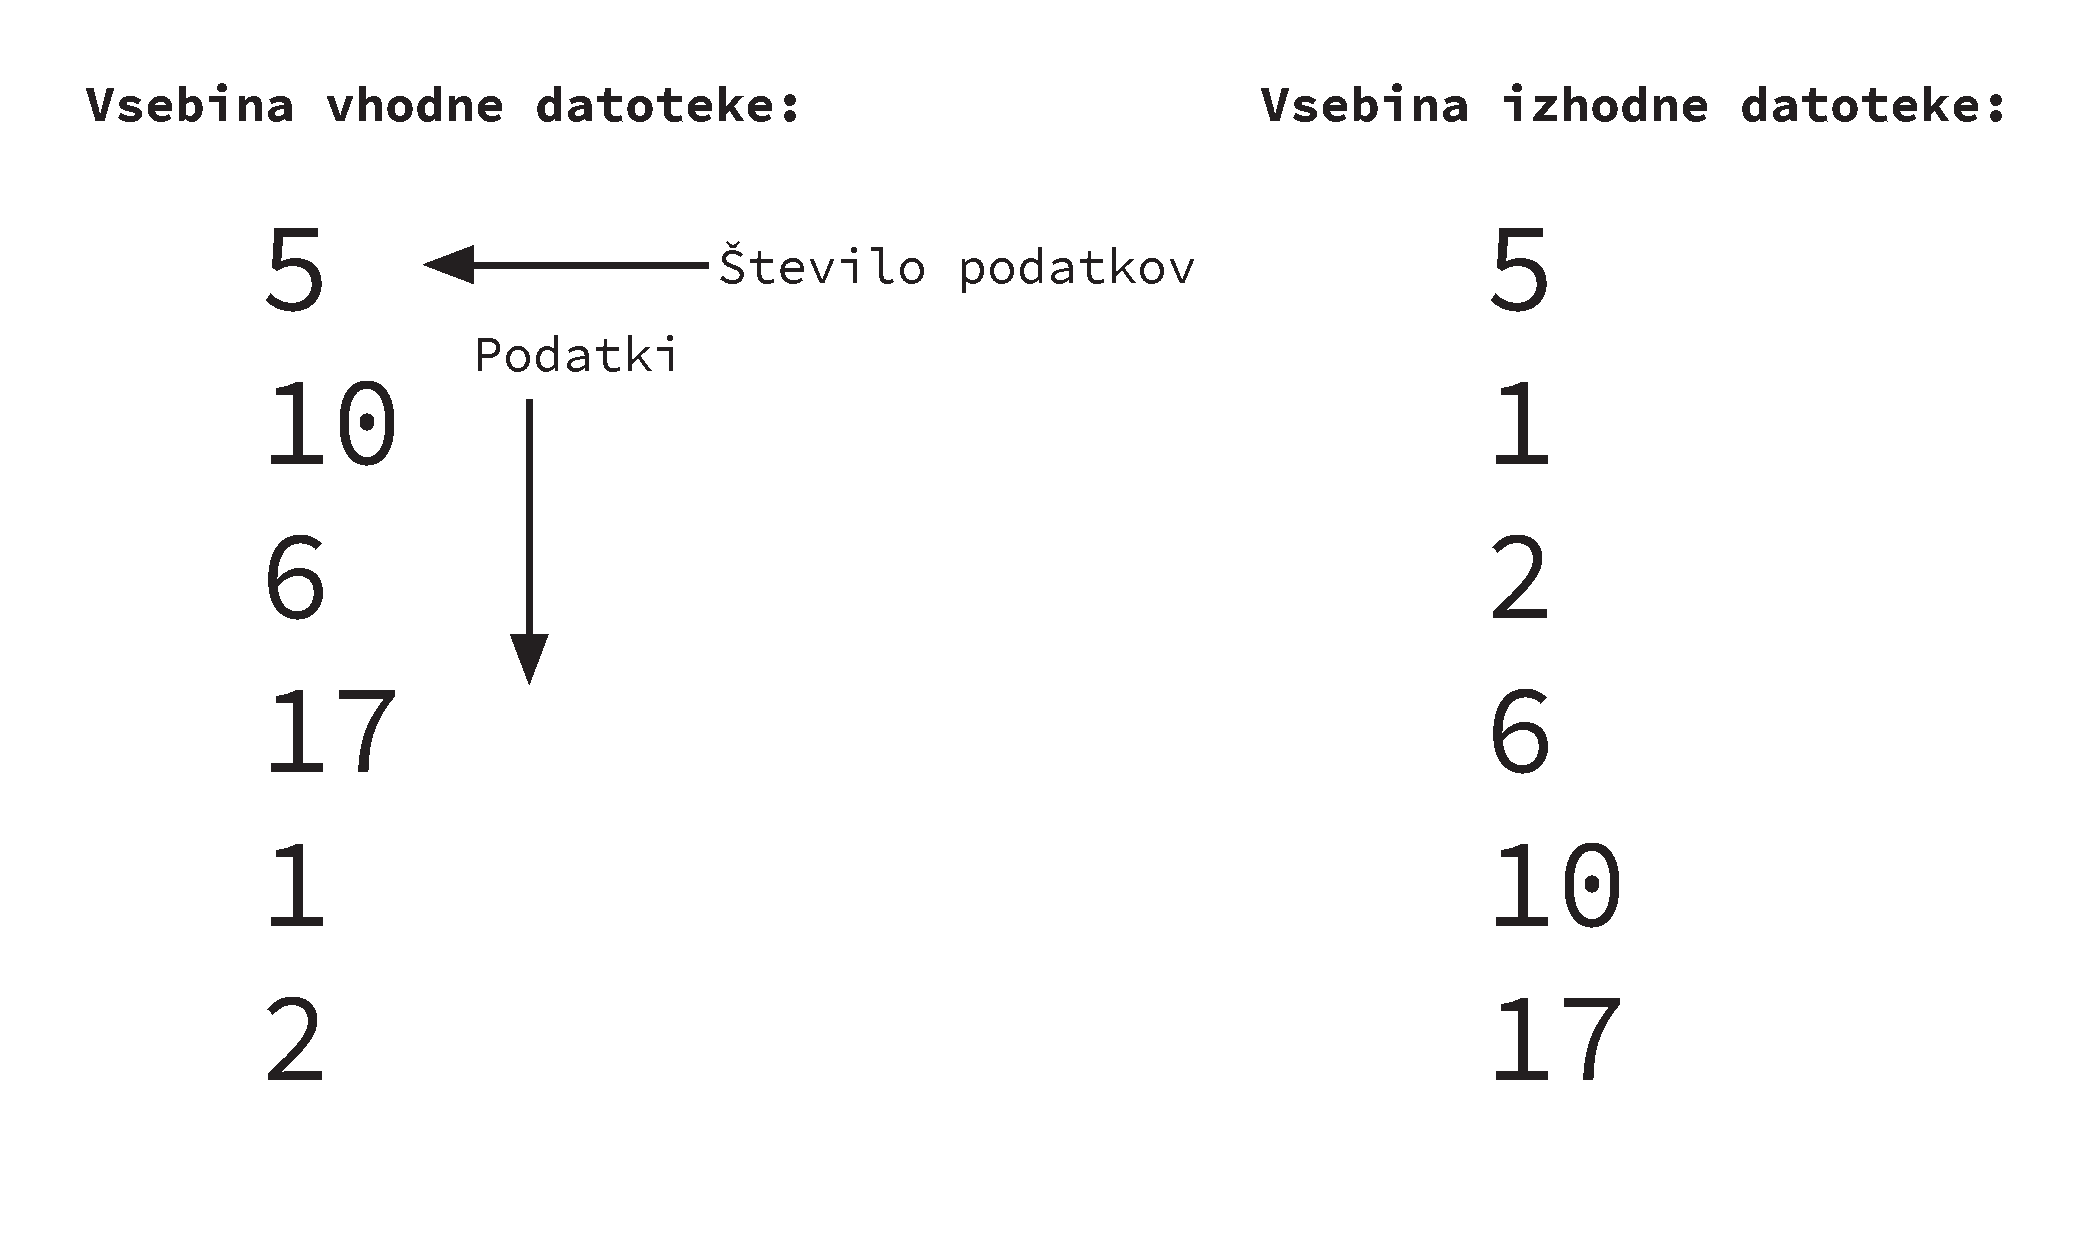
\includegraphics[width=0.75\textwidth]{8_ZZRS-sort_files.pdf}
  \caption{Slika prikazuje primer datoteke s katero operirata stre"znik in odjemalec.}
  \label{8_files}
\end{figure}

\subsection{Izbrani algoritmi za sortiranje}
\label{8_izbira_algoritmov}
Za namen testiranja smo implementirali dva algoritma. Najprej smo testirali z algoritmom za mehur"cno urejanje (ang. \textit{bubble sort}), ki ima "casovno zahevnost $O(n^2)$.
Da bi testirali vpliv izbire algoritma smo tudi implemenirali hitrej"si algoritem urejanja s porazdelitvami (ang. \textit{quicksort}), kateri ima povpre"cno "casovno zahtevnost $O(n* log(n))$.



\begin{minipage}[t]{0.45\linewidth}
\begin{lstlisting}[label={8_bubblesort},caption={Bubblesort}]

function bubblesort(int[] data){
	for(int i = 0; i < data.length;  i++){
		for(int j = 0; j < data.length; j++){
			if(data[i] < data[j]){
				int tmp = data[i];
				data[i] = data[j];
				data[j] = tmp;
			}
		}
	}
}

\end{lstlisting}
\end{minipage}
%
\begin{minipage}[t]{0.45\linewidth}
\begin{lstlisting}[label={8_quicksort}, caption={Quicksort}]

function quicksort(int[] data, int lo, int hi){
	if(lo < hi){
		int p = partition(data, lo, hi);
		quicksort(data, lo, p-1);
		quicksort(data, p+1, hi);
	}
}

function partition(int[] data, int lo, int hi){
	int pivot = data[hi];
	int i = lo -1;
	for(int j = lo; j < hi; j++){
		if(data[j] <= pivot){
			i = i+1;
			if(i != j){
				int tmp = data[i];
				data[i] = data[j];
				data[j] = tmp;
			}
		}
	}
	int tmp = data[i+1];
	data[i+1] = data[j];
	data[j] = tmp;
	return i+1;
}

\end{lstlisting}
\end{minipage}



\section{Izbira ponudnikov}
Najprej smo izbrali ponudnika obla"cnih storitev Cloud9, ki pa ni najbolj primeren za na"s problem, saj je v prvi vrsti razvojno okolje na spletu in se ne osredoto"ca na ponujanje stre"zni"ske infrastrukture. Pri ra"cunsko zahtevnej"sih testih smo naleteli na te"zave, saj je stre"znik po 120 sekundah povezavo zaprl. To je bil eden glavnih razlogov, da smo se odlo"cili za zamenjavo ponudnika obla"cnih storitev, saj smo le tako lahko izvedli vse "zeljene teste. Izbrali smo si ameri"sko podjetje DigitalOcean, ki je ponudnik istoimenske obla"cne infrastrukture. Na na"so sre"co sodelujejo v projektu Github Education Pack in tako "studentom nudijo 50\$ kredita za uporabo njihovih storitev.\\\\Svoje stre"znike imajo postavljene na slede"cih osmih lokacijah po svetu:
\begin{itemize}
\item New York (ZDA),
\item San Francisco (ZDA),
\item Amsterdam (Nizozemska),
\item Singapur (Singapur),
\item London (Zdru"zeno kraljestvo),
\item Frankfurt (Nem"cija),
\item Bangalore (Indija).
\end{itemize}
V okviru "studentskih kreditov so nam na voljo tri razli"cne konfiguracije, ki se med seboj razlikujejo po koli"cini dodeljenih resursov. Podatki o konfiguracijah so na voljo v tabeli \ref{8_table1}.

\begin{table}[!htbp]
  \centering
  \begin{tabular}{ | l | l | l | l | }
    \hline
    RAM & Stevilo procesorjev & Prostor na disku (SSD) & Cena na mesec\\ \hline
    512 MB & 1     & 20 GB &  5\$ \\ \hline
    1 GB & 1 & 30 GB & 10\$ \\ \hline
    2 GB & 2 & 40 GB & 20\$ \\ \hline
  \end{tabular}
  \caption{Konfiguracije stre"znikov, ki so na voljo za "studentske kredite.}
  \label{8_table1}
  \centering
\end{table}



\newpage
\section{Rezultati meritev}


\subsection{"Stevilo odjemalcev - Eksperiment 1}
\begin{itemize}
	\item \textbf{Hipoteza: }  \\
		Na"sa hipoteza je, da se povpre"cen "cas "cakanja odjemalca pribli"zno linearno pove"cuje z ve"canjem "stevila odjemalcev, ki hkrati po"siljajo datoteke na stre"znik.

	\item \textbf{Okoli"s"cine meritve: } \\
		Testiranje smo izvedli v "cetrtek 18.5.2017 med 21:00 in 21:30 na stre"zniku v Frankfurtu. Na stre"zniku je tekel operacijski sistem Linux Ubuntu 16.04. Na voljo smo imeli 512 MB RAM-a, 1 procesor ter 20 GB prostora na SSD trdem disku.\\Na stre"zniku je bil izbran algoritem za mehur"cno urejanje (ang. \textit{bubble sort}). Skripto za simulacijo odjemalcev smo pognali iz "studentskega naselja Ro"zna dolina (Ljubljana). Za dostop do interneta je bila uporabljena internetna povezana s hitrostjo 100 Mbps.\\ Na stre"znik so klienti (niti) po"siljali datoteke, ki so vsebovale 20,000 "stevil tipa integer in merili "case pri 1, 10, 20, 30 in 40 odjemalcih.

 	\item \textbf{Rezultati meritve: }  \\
	Rezultati meritve so vidni na sliki \ref{8_graf_1_rez}.
	\begin{figure}[!htb]
  	\centering
  	  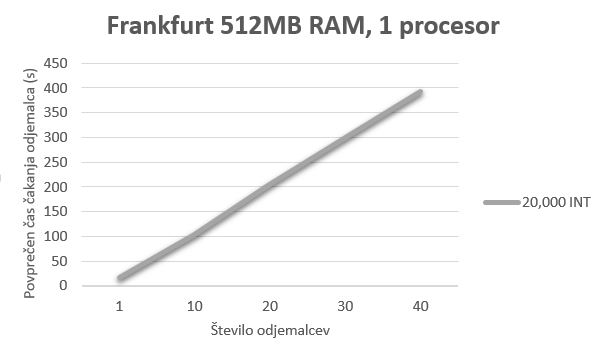
\includegraphics[width=1.0\textwidth]{8_test1_st_odjemalcev.jpg}
  	\caption{Graf povpre"cnega "casa "cakanja odjemalcev v odvisnosti od "stevila odjemalcev.}
  	\label{8_graf_1_rez}
	\end{figure}

	\begin{table}[!htbp]
  	\centering
  	\begin{tabular}{ | l | l | l | }
    	\hline
    	"Stevilo odjemalcev & Povpre"cni cas obdelave [s] & Standardna deviacija\\ \hline
    	1 & 16.06     & 0 \\ \hline
    	10 & 103.79 & 1.63\\ \hline
    	20 & 205.44 & 4.88\\ \hline
    	30 & 300.89 & 12.83\\ \hline
    	40 & 393.28 & 14.60\\ \hline
  	\end{tabular}
  	\caption{Tabela "casov obdelav datoteke z 20 tiso"c celimi "stevili.}
  	\label{8_table2}
  	\centering
	\end{table}

    \pagebreak
	\item \textbf{Komentar meritve: } \\
		Iz grafa~\ref{8_graf_1_rez} in tabele~\ref{8_table2} lahko zelo razlo"cno vidimo, da se z ve"canjem "stevila odjemalcev linearno pove"cuje tudi povpre"cen "cas "cakanja posameznega odjemalca. Opa"zen rezultat pri"cakovano sovpada z na"so hipotezo, saj ima stre"znik omejeno "stevilo resursov in morajo zato ob ve"cjem stevilu zahtevkov odjemalci  "cakati dlje. Prav tako lahko v tabeli opazimo, da se z ve"canjem "stevila odjemalcev pove"cuje tudi standardna deviacija, kar pa pomeni, da ob vi"sjih obremenitvah (ve"c odjemalcev) vedno te"zje predvidimo "cas obdelave datotek dolo"cenega odjemalca, saj prihaja do vedno ve"cjih odstopanj.
\end{itemize}

\newpage
\subsection{Velikost datotek - Eksperiment 2}
\label{8_subsec:eksperiment_2}
\begin{itemize}
	\item \textbf{Hipoteza: }  \\
		S slede"cim eksperimentom smo "zeleli preveriti odvisnost povpre"cnega "casa "cakanja klientov glede na velikost datotek. Da bi izni"cili vpliv "stevila odjemalcev na ta poizkus smo teste ponovili na ve"c razli"cnih "stevilih odjemalcev. V tem primeru predpostavljamo hipotezo, da se z ve"canjem velikosti datoteke ve"ca tudi povpre"cni "cas "cakanja klientov.

	\item \textbf{Okoli"s"cine meritve: } \\
		Testiranje smo izvedli v "cetrtek 18.5.2017 med 21:30 in 24:00 na stre"zniku v Frankfurtu. Na stre"zniku je tekel operacijski sistem Linux Ubuntu 16.04. Na voljo smo imeli 512MB RAM-a, 1 procesor ter 20GB prostora na SSD trdem disku.\\ Na stre"zniku je bil izbran algoritem za mehur"cno urejanje (ang. \textit{bubble sort}). Skripto za simulacijo odjemalcev smo pognali iz "studentskega naselja Ro"zna dolina (Ljubljana). Za dostop do interneta je bila uporabljena internetna povezana s hitrostjo 100 Mbps.\\ Na stre"znik so klienti (niti) po"siljali datoteke, ki so vsebovale velikosti 10,000, 15,000, 20,000, 25,000, 30,000, 40,000 in 50,000 "stevil tipa integer. Meritve smo ponovili na 1, 10, 20, 30 in 40 odjemalcih.

 	\item \textbf{Rezultati meritve: }  \\

    \begin{table}[!h]
      \centering
        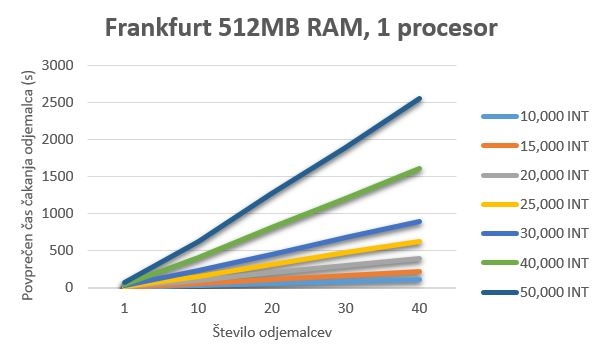
\includegraphics[width=1.0\textwidth]{8_test2_velikost_datotek.jpg}
      \caption{Graf povpre"cnega "casa "cakanja odjemalcev v odvisnosti od velikosti datotek.}
      \label{8_graf_2_rez}
    \end{table}

    \pagebreak
	\item \textbf{Komentar meritve: } \\
		Iz grafa na sliki ~\ref{8_graf_2_rez} zelo razlo"cno vidimo, da se povpre"cen "cas "cakanja posameznega odjemalca z ve"canjem velikosti datotek zelo hitro pove"cuje. Pri 40 odjemalcih in datoteki velikosti 10,000 "stevil tipa integer je povpre"cni "cas "cakanja pribli"zno 170 sekund. Pri datoteki veliosti 50,000 "stevil pa ta "cas zna"sa "ze ve"c kot 2550 sekund. To je bilo pri"cakovano, saj je bil za urejanje "stevil uporabljen algoritem za mehur"cno urejanje (bubble sort), ki ima "casovno zahtevnost $O(n^2)$. Rezultati tega eksperimenta potrdijo, da se tudi na oblaku potreben "cas za obdelavo datotek z algoritmom \textit{bubble sort} pove"cuje pribli"zno s kvadratom velikosti datotek.
\end{itemize}

\newpage
\subsection{Ozko grlo na stre"zniku - Eksperiment 3}
\begin{itemize}
	\item \textbf{Hipoteza: }  \\
		Z na"simi meritvami smo stre"znike obremenili do najvi"sjih dovoljenih meja. V praksi ob maksimalni obremenitvi sistema vedno obstaja neko ozko grlo sistema, ki ne more delovati hitreje in s tem zni"zuje hitrosti delovanja sistema celotnega sistema. V na"sem primeru predpostavljamo, da je najbolj obremenjena komponenta procesor, saj je sortiranje operacija, ki zahteva relativno veliko ra"cunskih operacij(predvsem primerjanj).

	\item \textbf{Okoli"s"cine meritve: } \\
		Obremenitve stre"znika smo merili med Eksperimentom 2 (poglavje \ref{8_subsec:eksperiment_2}).

 	\item \textbf{Rezultati meritve: }  \\
		\begin{figure}[!htb]
  		\centering
  		  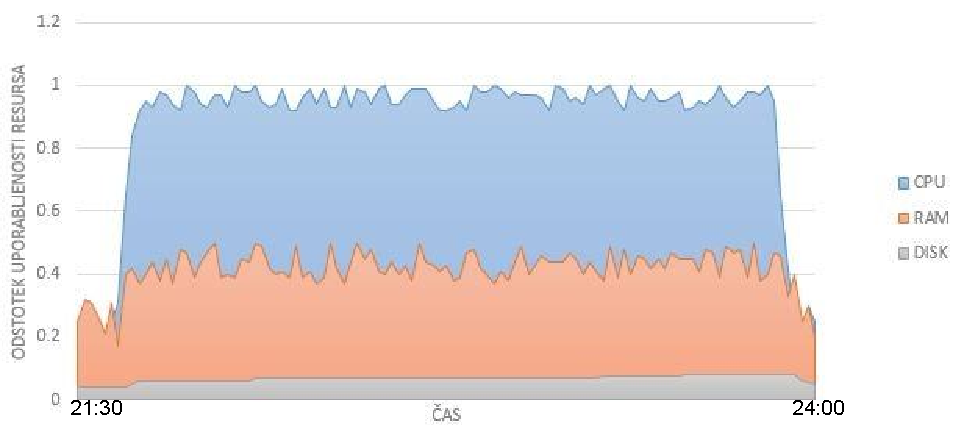
\includegraphics[width=1.0\textwidth]{8_test3_resursi.pdf}
  		\caption{Graf zasedenosti resursov med izvajanem testovs.}
  		\label{8_graf_zasedenost_resursov}
		\end{figure}


	\item \textbf{Komentar meritve: } \\
		Iz slike \ref{8_graf_zasedenost_resursov} lahko razlo"cno razberemo, da je ozko grlo na"sega sistema procesor, saj je prakti"cno ves "cas izvajanja testov 100\% obremenjen. Poraba RAM-a in kapacitete trdega diska niso nikoli ekstremno obremenjene, saj med izvajanjem nikoli ne uporabljamo ve"c kot 50\% RAM-a. Razlog za majhno porabo RAM-a je v tem, da odjemalci "cakajo na odgovor stre"znika pred po"siljanjem novih datotek. Tudi v primeru, ko odjemalci ne "cakajo, pa nam ni uspelo dose"ci dovolj visoke zasedenosti, da bi zru"sili sistem. Razloga za to sta omejeno "stevilo niti na odjemalcu ter omejeno "stevilo hkrati odprtih datotek na odjemalcu. Zasedenost diska pa je prakti"cno zanemarljiva, saj so datoteke relativno majhne glede na ponujeno velikost trdega diska, datoteke pa se sproti bri"sejo in tako prepre"cimo te"zave z prezasedenostjo trdega diska.
\end{itemize}

\newpage
\subsection{Lokalnost - Eksperiment 4}
\label{8_subsec:eksperiment_4}
\begin{itemize}
	\item \textbf{Hipoteza: }  \\
		Zaradi mo"znosti izbire lokacije stre"znika smo "zeleli preveriti vpliv lokacije na povpre"cni "cas "cakanja odjemalcev. Poleg stre"znika v Frankfurtu smo vzpostavili tudi stre"znik v San Franciscu. Predvidevamo, da bomo hitrej"se odzive dobivali od stre"znika v Frankfurtu, saj nam je fizi"cno precej bli"ze, kot San Francisco.
	\item \textbf{Okoli"s"cine meritve: } \\
		Stre"znika imata dodeljeno enako koli"cino resursov in name"s"ceno identi"cno programsko opremo. Ta je enaka kot v testu 2 (poglavje \ref{8_subsec:eksperiment_2}) Slednje je bilo potrebno zagotoviti, da izklju"cimo vpliv programske opreme na hitrost odziva stre"znika. Testiranje smo izvedli v ponedeljek 22.5.2017 med 10:00 in 14:00 po "casu UTC+01:00. Zaradi "casovnih pasov je bila ura v San Franciscu v "casu testiranja med 1:00 in 5:00 zjutraj. Teste smo ponovili z datotekami velikosti 20,000 in 50,000 celih stevil.

 	\item \textbf{Rezultati meritve: }  \\
		\begin{figure}[h]
  		\centering
  		  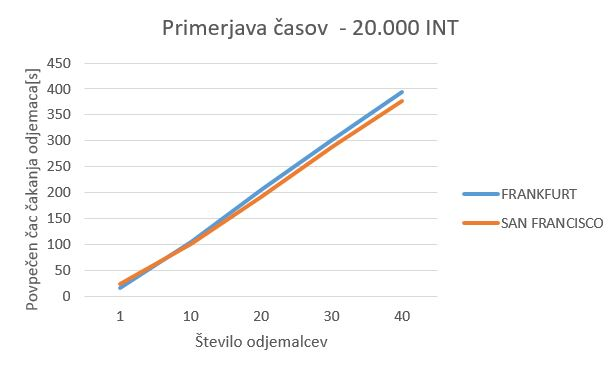
\includegraphics[width=1.0\textwidth]{8_test4_lokalnost_20.jpg}
  		\caption{Graf povpre"cnega "casa cakanja odjemalcev v odvisnosti od lokacije na primeru datoteke z 20,000 "stevili}
  		\label{8_graf_lokalnost_20}
		\end{figure}

		\begin{figure}[h]
  		\centering
  		  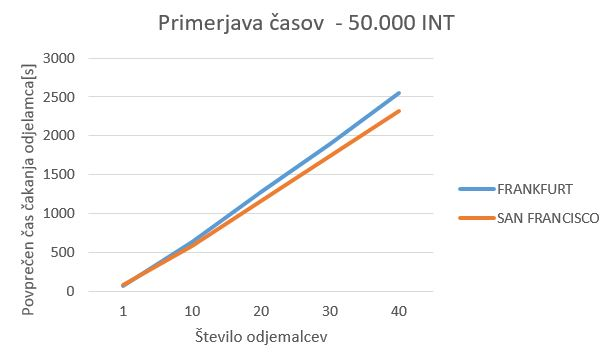
\includegraphics[width=1.0\textwidth]{8_test4_lokalnost_50.jpg}
  		\caption{Graf povpre"cnega "casa cakanja odjemalcev v odvisnosti od lokacije na primeru datoteke z 50,000 "stevili}
  		\label{8_graf_lokalnost_50}
		\end{figure}

    \newpage
	\item \textbf{Komentar meritve: } \\
		Rezultati meritev iz slik \ref{8_graf_lokalnost_20} in \ref{8_graf_lokalnost_50} niso potrdili na"se hipoteze, saj se je stre"znik v San Franciscu kljub ve"cji oddaljenosti hitreje odzival in vra"cal urejene datoteke.
		Razlike so vse bolj opazne ob ve"cji obremenitvi sistema (ve"cje datoteke in ve"c odjemalcev). Pri datoteki velikost 20,000 "stevil in enem odjemalcu lahko vidimo, da nam rezultate hitreje vrne stre"znik v Frankfurtu. Rezultate si razlagamo na na"cin, da je bil stre"znik v Frankfurtu bolj obremenjen v "casu izvajanja testov. Pri majhnih primerih je kljub svoji obremenjenosti uspel rezultat vrniti pred stre"znikom v San Franciscu. Z ve"canjem ra"cunske zahtevnosti problema pa je vse bolj do izraza pri"sla manj"sa zasedenost infrastrukture v San Franciscu. Drug mo"zen razlog bi lahko bili zmogljivej"si procesorji v stre"znikih lociranih v San Franciscu, vendar interne informacije o zgradbi stre"zni"skih centrov "zal niso javne.
\end{itemize}

\newpage
\subsection{Razli"cne ra"cunske mo"ci - Eksperiment 5}
\begin{itemize}
	\item \textbf{Hipoteza: }  \\
		Na"sa hipoteza, ki jo bomo prevelili v tem poizkusu pravi, da se povpre"cni "cas "cakanja odjemalcev bistveno zmanj"sa, "ce je stre"znik bolj zmogljiv(ve"c procesorjev in RAM-a).

	\item \textbf{Okoli"s"cine meritve: } \\
		Testiranje smo izvedli v torek 23.5.2017 med 00:30 in 02:30 na stre"zniku v Frankfurtu. Na stre"zniku je tekel operacijski sistem Linux Ubuntu 16.04. Na voljo smo imeli 2 GB RAM-a ter 2 procesorja. Na stre"zniku je bil izbran algoritem za mehur"cno urejanje (ang. \textit{bubble sort}).\\ Skripto za simulacijo odjemalcev smo pognali iz "studentskega naselja Ro"zna dolina(Ljubljana). Za dostop do interneta je bila uporabljena internetna povezana s hitrostjo 100Mbps.\\ Na stre"znik so klienti (niti) po"siljali datoteke velikosti 20,000 in 50,000 "stevil tipa integer in merili "case pri 1, 10, 20, 30 in 40 odjemalcih.

 	\item \textbf{Rezultati meritve: }  \\

		V grafih na slikah \ref{8_graf_racunska_moc_20} in \ref{8_graf_racunska_moc_50} so vizualizani povpre"cni "casi odziva treh razli"cnih streznikov. Stre"znik Frankfurt1 in San Francisco imata identi"cno konfiguracijo, kot je opisana v eksperimentu 4 (poglavje \ref{8_subsec:eksperiment_4}). Stre"znik Frankfurt2 pa ima na voljo 2 procesorja ter 2 GB RAM-a.

		\begin{figure}[h]
  		\centering
  		  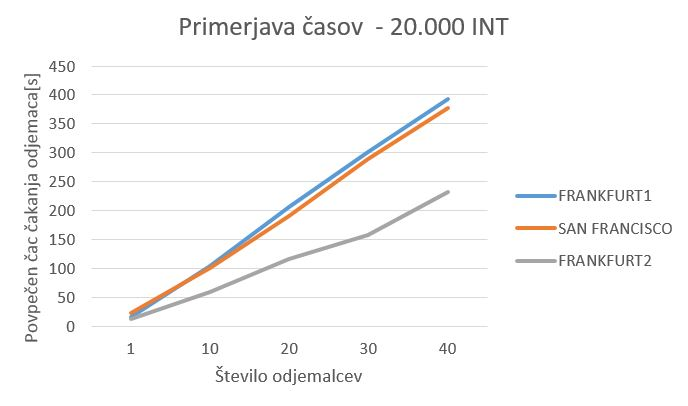
\includegraphics[width=1.0\textwidth]{8_test5_racunska_moc_20.jpg}
  		\caption{Graf povpre"cnega "casa "cakanja odjemalcev treh razli"cnih stre"znikov na primeru datotek z 20,000 "stevili.}
  		\label{8_graf_racunska_moc_20}
		\end{figure}

	\begin{figure}[h]
  		\centering
  		  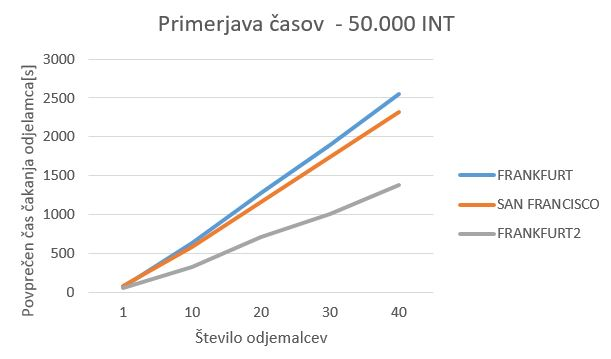
\includegraphics[width=1.0\textwidth]{8_test5_racunska_moc_50.jpg}
  		\caption{Graf povpre"cnega "casa "cakanja odjemalcev treh razli"cnih stre"znikov na primeru datotek s 50,000 "stevili.}
  		\label{8_graf_racunska_moc_50}
		\end{figure}
	\item \textbf{Komentar meritve: } \\
		Meritve potrdijo na"so predpostavko, da vi"sja zmogljivost stre"znikov pripomore k bistveno ni"zjim povpre"cnim "casom potrebnim za odziv.
\end{itemize}

\newpage
\subsection{24 urni test - Eksperiment 6}
\begin{itemize}
	\item \textbf{Hipoteza: }  \\
		Zaradi ugotavljanja zasedenosti omre"zja ter stre"znikov smo izvedli "se 24 ur trajajo"ci test. Na"sa predpostavka je, da bodo "casi odzivov vi"sji v dnevnih "casovnih razmerah, tj. "cez dan kot pa pono"ci.

	\item \textbf{Okoli"s"cine meritve: } \\
		Testiranje smo izvedli v petek 26. in v soboto 27.5.2017. Test smo za"celi izvajatvi v petek ob 13:30 in smo ga izvajai 24 ur na stre"zniku v Frankfurtu. Na stre"zniku je tekel operacijski sistem Linux Ubuntu 16.04. Na voljo smo imeli 2GB RAM-a, 2 procesorja ter 40 GB prostora na SSD trdem disku. Na stre"zniku je bil izbran algoritem za mehur"cno urejanje (ang. \textit{bubble sort}).\\ Skripto za simulacijo odjemalcev smo pognali v Trzinu. Za dostop je bila uporabljena internetna ponudba Telekom Slovenije s hitrostjo 20Mbps.\\ Na stre"znik so klienti (niti) po"siljali datoteke velikosti 20,000 celih "stevil za sortiranje v intervalih po 300 sekund. Slednje je po"celo 20 odjemalcev hkrati. Merili smo povpre"cen ca"s "cakanja odjemalcev in kako se ta spreminja skozi celoten dan.

 	\item \textbf{Rezultati meritve: }  \\
		\begin{figure}[h]
  		\centering
  		  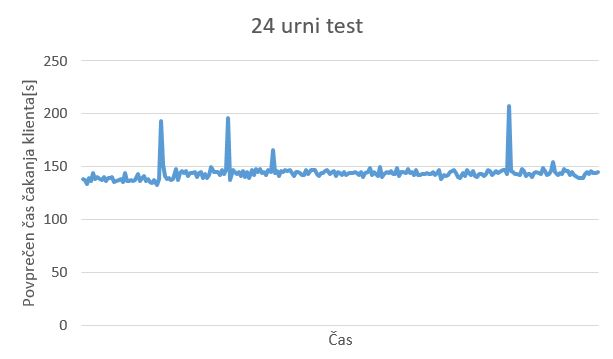
\includegraphics[width=1.0\textwidth]{8_test6_24h.jpg}
  		\caption{Graf povpre"cnega "casa cakanja odjemalcev v 24 urah }
  		\label{8_graf_racunska_moc_50}
		\end{figure}

	\item \textbf{Komentar meritve: } \\
		Z meritvijo smo ugotovili, da je povpre"cen "cas "cakanja odjemalcev preko celega dneva prakti"cno enak. To si razlagamo tako, da stre"zniki nikoli niso tako obremenjeni, da bi to vplivalo na odzivne "case. "Cas prena"sanja datotek pa zaradi razmeroma hitrih internetnih povezav predstavlja manj"si dele"z skupnega "casa. Iz povpre"cja bolj o"citno odstopajo le "stiri meritve, ki so trajale ob"cutno dalj "casa. Te meritve pa nam ne povedo veliko uporabnega, saj so razporejene dokaj naklju"cno "cez celoten dan. Na"sa hipoteza, ki predpostavlja, da bodo "casi obdelave sredi dneva ob"cutno vi"sji od tistih pono"ci je bila napa"cna.
\end{itemize}

    \subsection{Izbira algoritma - Eksperiment 7}
    \begin{itemize}
    	\item \textbf{Hipoteza: }  \\
    		Na strani stre"znika smo za implementirali dva razli"cna algoritma za urejanje "stevil opisana v podpoglavju \ref{8_izbira_algoritmov} . V tem eksperimentu bomo iste naklju"cne datoteke po"siljali na stre"znik ter merili "case do prejema datotek pri obeh algoritmih.
		Na"sa hipoteza je, da bo stre"znik na katerem te"ce algoritem \textit{quicksort} z nalogo opravil veliko hitreje, kot stre"znik z izbranim algoritmom \textit{bubblesort}.

    	\item \textbf{Okoli"s"cine meritve: } \\
    		Testiranje smo izvedli v sredo 31.5.2017 med 15:00 in 16:00 na stre"zniku v Frankfurtu. Na stre"zniku je tekel operacijski sistem Linux Ubuntu 16.04. Na voljo smo imeli 2 GB RAM-a ter 2 procesorja. Skripto za simulacijo odjemalcev smo pognali iz "studentskega naselja Ro"zna dolina(Ljubljana). Za dostop do interneta je bila uporabljena internetna povezana s hitrostjo 100Mbps.\\ Na stre"znik so klienti (niti) po"siljali datoteke velikosti 20,000 "stevil tipa integer in merili "case pri 1, 10, 20, 30 in 40 odjemalcih.

     	\item \textbf{Rezultati meritve: }  \\
		Na sliki \ref{8_graf_algorithms} lahko vidimo gafi"cno predstavljene rezultate meritve.
    		\begin{figure}[h]
  		\centering
  		  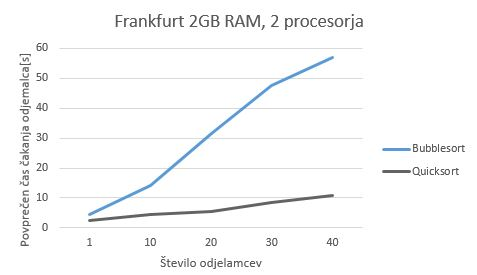
\includegraphics[width=1.0\textwidth]{8_test_frankfurt_algorithms.jpg}
  		\caption{Graf povpre"cnega "casa cakanja odjemalcev pri razli"cnih algoritmih }
  		\label{8_graf_algorithms}
		\end{figure}
    		\newpage

    	\item \textbf{Komentar meritve: } \\
    		Rezultati vidni na sliki  \ref{8_graf_algorithms} potrjujejo na"so hipotezo. "Cas sortiranja na stre"zniku na naklju"cnih datotekah je precej manj"si ob uporabi algoritma \textit{quicksort}.
    \end{itemize}


\subsection{Zlom sistema - Eksperiment 8}
    \begin{itemize}
    	\item \textbf{Hipoteza: }  \\
    		Za konec smo "zeleli tudi zlomit sistem oz. ga prisiliti v to, da nam ne vra"ca ve"c pravilnih rezultatov. Na"sa hipoteza je, da bomo prej ali slej pri"sli do to"cke, ko bo stre"znik zaradi predolgega trajanja povezavo zaprl.

    	\item \textbf{Okoli"s"cine meritve: } \\
    			Testiranje smo izvedli v "cetrtek 1.6.2017 med 19:00 in 20:30 na stre"zniku v Frankfurtu. Na stre"zniku je tekel operacijski sistem Linux Ubuntu 16.04. Na voljo smo imeli 512MB RAM-a ter 1 procesor. Na stre"zniku je bil izbran algoritem za mehur"cno urejanje (ang. \textit{bubble sort}).\\ Skripto za simulacijo odjemalcev smo pognali iz "studentskega naselja Ro"zna dolina(Ljubljana). Za dostop do interneta je bila uporabljena internetna povezana s hitrostjo 100Mbps.\\ Na stre"znik so klienti (niti) po"siljali datoteke velikosti 50,000  "stevil tipa integer in merili "case pri 1, 10, 20, 30, 40, 50, 60 in 80 odjemalcih.

     	\item \textbf{Rezultati meritve: }  \\
    		\begin{figure}[h!]
  		\centering
  		  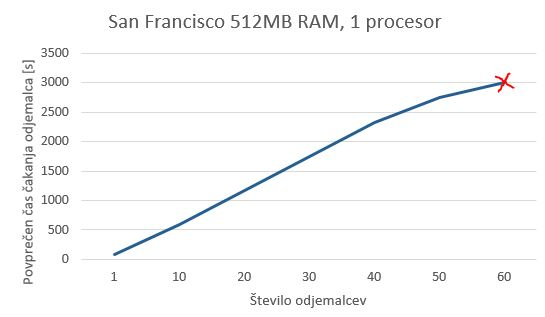
\includegraphics[width=1.0\textwidth]{8_test_zlom_sistema.jpg}
  		\caption{Graf povpre"cnega "casa cakanja odjemalcev pri uspe"snem poizkusu zloma sistema. }
  		\label{8_graf_zlom_sistema}
		\end{figure}
    		 \newpage
    	\item \textbf{Komentar meritve: } \\
    		Z eksperimentom, ki je prikazan na sliki \ref{8_graf_zlom_sistema}, nam je uspelo uspe"sno dose"ci zlom sistema, saj je stre"znik po pribli"zno 3000 s "cakanja na odgovor povezavo prekinil. Podrobnej"se sporo"cilo o napaki je na vojo v listingu \ref{8_error_report}.
		Ker nismo vedeli na kak"sen nacin in kdaj bo pri"slo do zloma stre"znika je bilo potrebno veliko poizkusov, da smo dosegli "zeljen rezultat.

\lstset{label={8_error_report},caption={Napaka ob zlomu sistema},language=Bash}
	\begin{lstlisting}
Traceback (most recent call last): File "C:\Anaconda3\lib\site-packages\requests\adapters.py", line 324, in send timeout=timeout
  File "C:\Anaconda3\lib\site-packages\requests\packages\urllib3\ connectionpool.py", line 528, in urlopen raise MaxRetryError(self, url, e)
requests.packages.urllib3.exceptions.MaxRetryError: HTTPConnectionPool(host='139.59.132.145', port=8080): Max retries exceeded with url: /nalozi (Caused by <class 'TimeoutError'>: [WinError 10060] A connection attempt failed because the connected party did not properly respond after a period of time, or established connection failed because connected host has failed to respond)
	\end{lstlisting}

    \end{itemize}


\section{Zaklju"cek}

Na"s cilj je bil preveriti zmogljivost obla"cnih storitev za izvajanje ra"cunsko zahtevnih operacij. Uporabili smo stre"zni"sko infrastrukturo podjetja DigitalOcean in na njej izvajali operacijo urejanja "stevil, saj ta vsebuje veliko operacij(primerjanj).
Izvajali smo razli"cne teste, ter tako preverjali vpliv dolo"cenih spremenljivk na zmogljivost na"sega sistema. \\
S testi smo hoteli ugotoviti vplive "stevila odjemalcev, velikosti datotek, lokacije stre"znika, koli"cine razpolo"zljivih resursov na stre"zniku, dela dneva ter izbire algoritma na hitrost odziva stre"znika. Poleg tega smo izvedli tudi test s katerim smo povzro"cili zlom sistema.
Merili smo predvsem "case potrebne za po"siljanje in sortiranje datotek ter zasedenost resursov na stre"zniku.\\
Kot glavno ozko grlo stre"znika se je pri"cakovano izkazal CPU, saj mora pri sortiranju opraviti zelo veliko operacij primerjanja. Maksimalno zasedenost CPU-ja laho hitro dose"zemo z ve"canjem "stevila odjemalcev in velikosti datotek.\\
Za metrike smo se odlo"cili na podlagi "clanka \cite{8_ibm_metrics}. V veliko pomo"c pa so nam bile tudi ugotovitve iz "clankov \cite{8_performance_challenges}, \cite{8_performance_analysis} in \cite{8_performance_evaluation}.

Na podlagi eksperimentov smo ugotovili, da je izbira algoritma zelo pomembna in bistveno vpliva na "cas obdelave. Prav tako je klju"cna obremenjenost stre"znika s "stevilom klientov.
Kljub vsemu, pa stre"znik s tako nizkimi zmogljivostmi ne pride v po"stev za prakti"co uporabo re"sevanja ra"cunskih problemov namesto kon"cnih delovnih tock(osebnih ra"cunalnikov). Ob tem pa je potrebno poudariti, da na trgu obstajajo tudi precej
zmogljivej"se re"sitve, ki omogo"cajo bistveno ve"cjo ra"cunsko mo"c. Vedno hitrej"si stre"zniki in pove"cevanje povpre"cne hitrosti internetne povezave, pa bo slej ko prej pripeljalo do to"cke, ko bomo iz kon"cnih to"ck ra"cunsko zahtevne probleme v obdelavo po"siljali na stre"znik. Na"se naprave, pa bodo skrbele le za interakcijo s stre"znikom in prikaz rezultatov. 
